\section{Experiments}

We subsequently apply our method to ligand-binding pocket classification, a $7$-classification task. The loss function was selected to be the cross-Entropy loss.

\begin{figure}[htp]
    \centering
    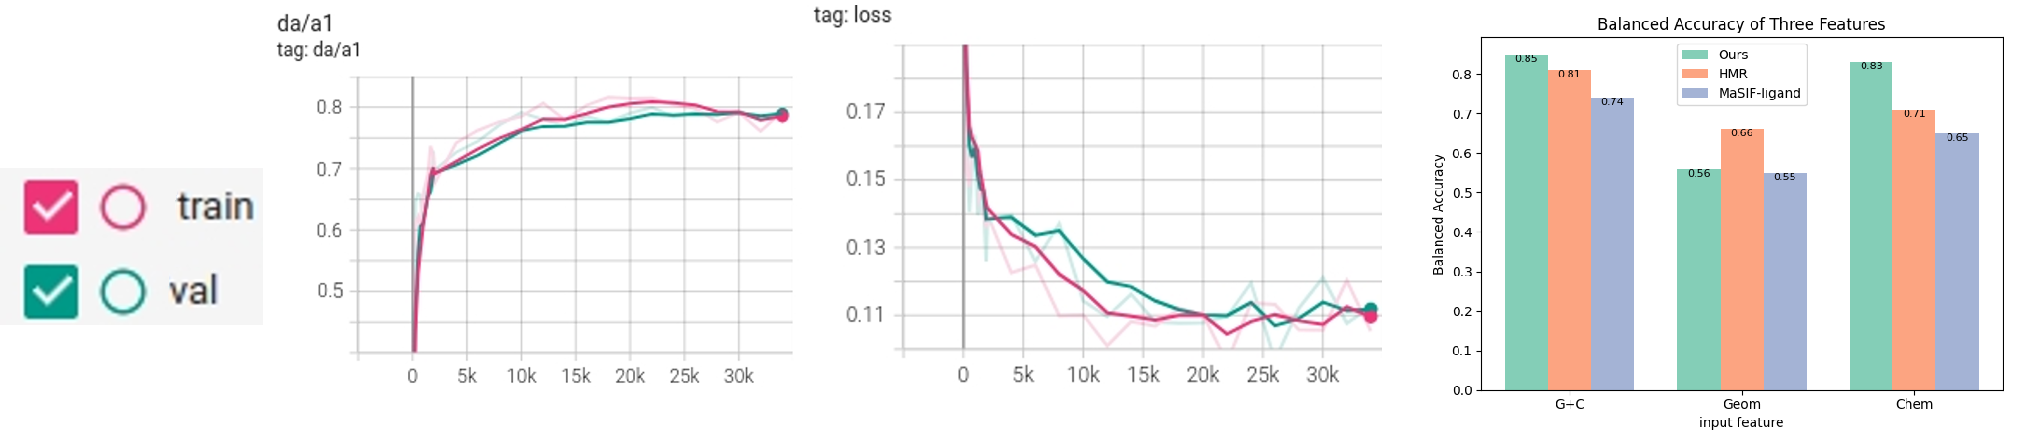
\includegraphics[width=\linewidth]{figures/result.png}
    \caption{
        Balanced accuracy of ligand-binding protein pocket classification.
        Models with different input features are compared: ``G+C'' indicates both geometric and chemical features.
    }
    \label{fig:ligand-binding-result}
\end{figure}

The dataset provided in MaSIF \cite{MaSIF} comprises computed properties of protein surfaces, crucial for understanding protein interactions with other molecules. These properties are utilized to discern patterns or "fingerprints" of interaction based on geometric and chemical features of the molecular surface. These fingerprints are then employed to predict how a given protein might interact with other proteins, ligands, or pharmaceuticals, enhancing insights into biological processes and assisting in drug design. Specifically, each protein in the dataset is associated with a preferred ligand-binding type among seven options (ADP, COA, FAD, HEM, NAD, NAP, and SAM). We consider the hydrophobicity score and partial charge as chemical features and mean/Gaussian curvature and Heat Kernel Signatures as geometric features. The dataset comprises 1634 training cases, 202 validation cases, and 418 testing cases.
\paragraph{Model Architecture}
Model Architecture and Performance 
The LBSR-based classification method contains 6 propagation layers followed by a global average pooling layer to aggregate information from all surface points of a ligand-binding pocket. A simple two-layer MLP is used to classify pockets into one of the seven ligand-binding pockets mentioned above.
LBSR has been trained to minimize the cross-entropy loss for 400 epochs and the one with the best balanced accuracy score on the validation set is selected.
\paragraph{Results}
Our result is shown in Figure \ref{fig:ligand-binding-result}. It suggests that our representation outperforms the 3D CNN-based methods used in MaSIF \cite{MaSIF}. It effectively encodes both the geometric and chemical features to predict protein binding type classification.